\section{Verhaltensdarstellung über Komplexe Zahlen}
Normalerweise werden komplexe Zahlen via der imaginären Einheit $\imu^2 \coloneqq -1$ eingeführt.
Anschließend definiert man dann die komplexen Zahlen über $\mathbb{C} \ni c \coloneqq a + b\cdot \imu$ mit $a,b \in \mathbb{R}$.
Aus dieser Herangehensweise folgen dann recht schnell die Regeln zum Rechnen mit ebendiesen.
\begin{align*}
    c_1 +c_2 &= (a_1 + b_1\cdot \imu) + (a_2 + b_2\cdot \imu) &
    c_1 \cdot c_2 &= (a_1 + b_1\cdot \imu) \cdot (a_2 + b_2\cdot \imu) \\
        &= (a_1 + a_2) + (b_1 + b_2)\cdot \imu  &
        &= a_1a_2 + b_1b_2 \cdot \imu^2 + a_1b_2 \cdot \imu + a_2b_1 \cdot \imu\\
        &&&= (a_1a_2 - b_1b_2) + (a_1b_2 + a_1b_2) \cdot \imu
\end{align*}

\begin{wrapfigure}{r}{0.4\textwidth}
  \begin{centering}
    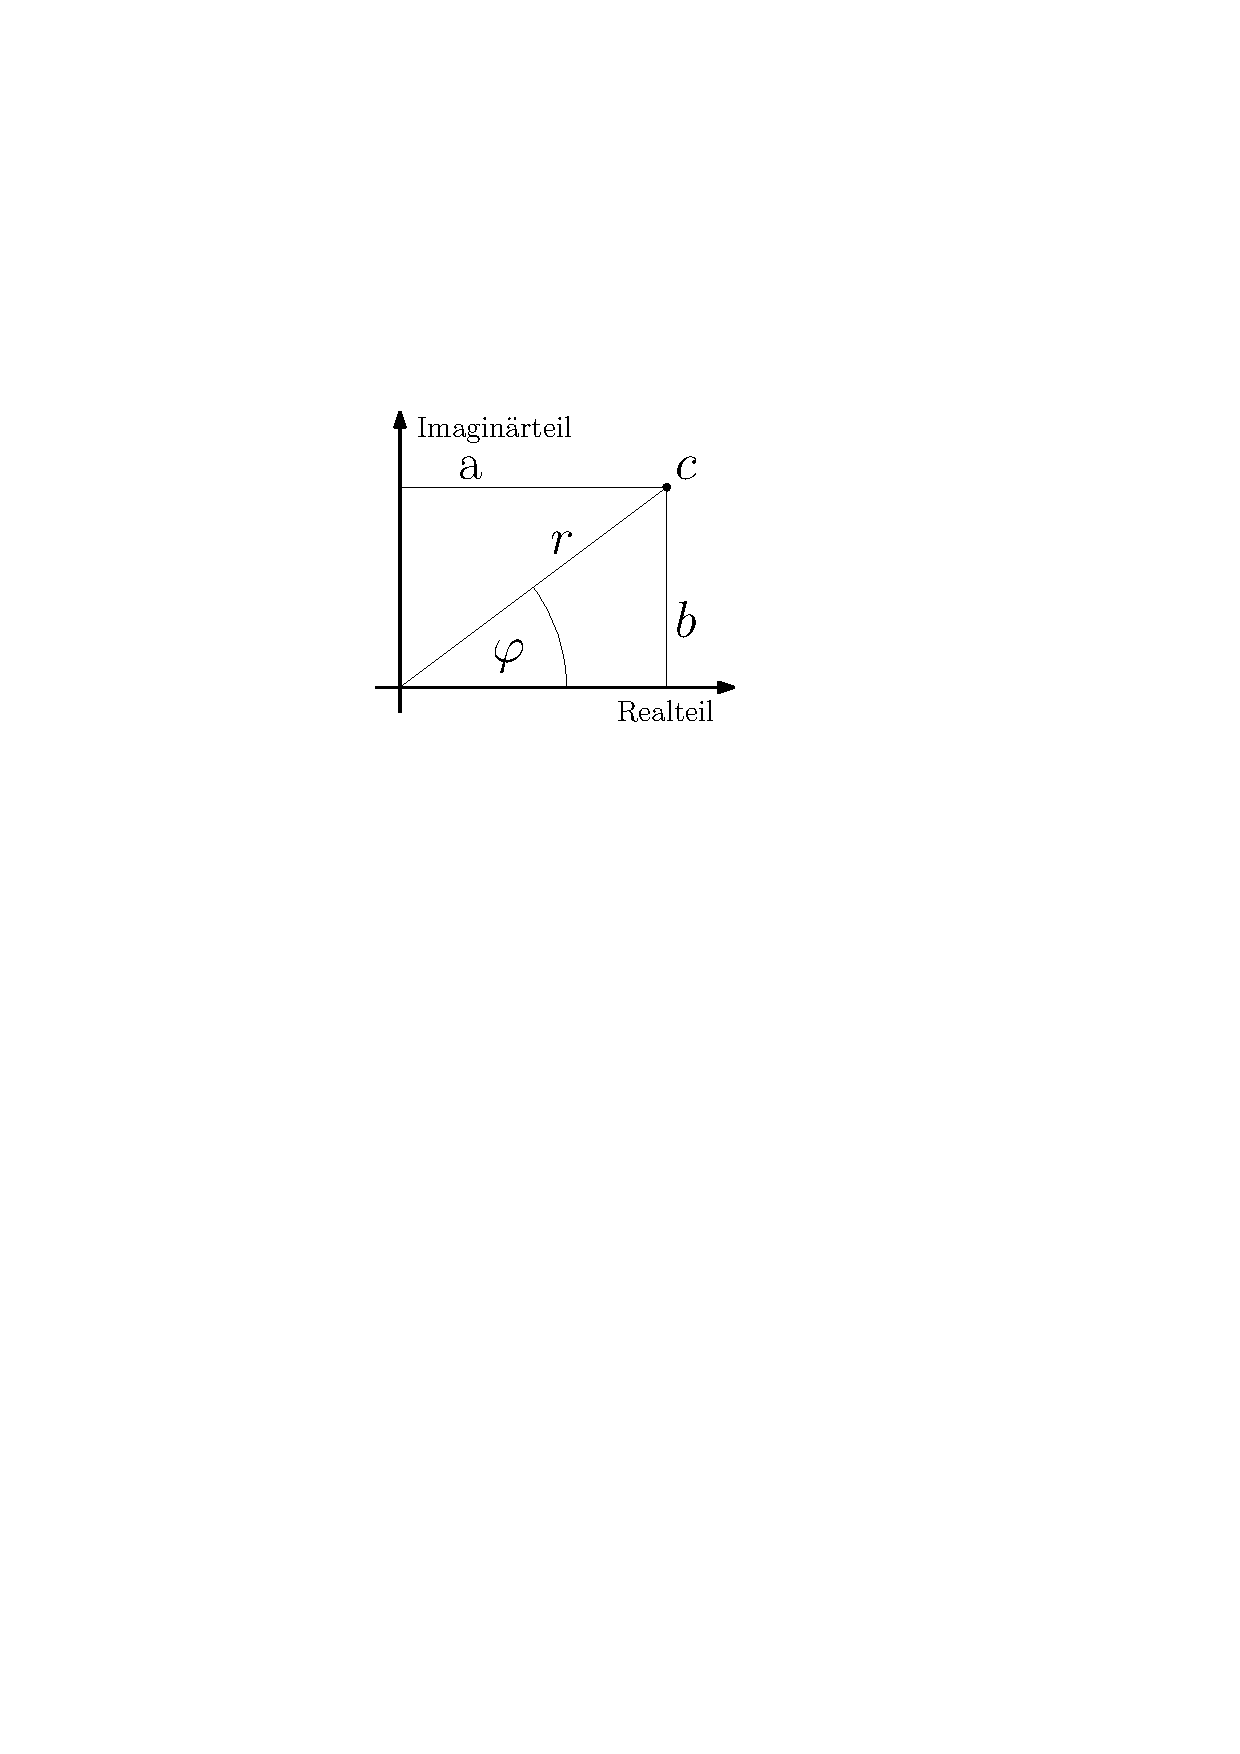
\includegraphics[width=0.4\textwidth]{philip1.pdf}
  \end{centering}
  \caption{Komplexe Zahl $c$ in kartesischen und polaren Koordinaten}
\end{wrapfigure}

Für den Anwendungsbereich der Wechselstromberechnungen ist es jedoch sinnvoller, komplexe Zahlen als
Repräsentanten von Punkten im zweidimensionalen Raum zu sehen, welche über die oben genannten Rechenvorschriften nützliche Eigenschaften besitzen, auf die im folgenden eingegangen werden soll.

Man denke sich eine komplexe Zahl $a +b\imu$ als einen Vektor $(a,\,b)_{x,y}$ im kartesischen Koordinatensystem mit X- und Y-Achse.
Dann sieht man, dass die Addition zweier komplexer Zahlen genau der Vektoraddition entspricht.
Weiterhin kann man den Vektor auch in einem polaren Koordinatensystem darstellen, in dem man aus $a$ und $b$ den 
Abstand zum Koordinatenursprung $r$ und den Winkel zur X-Achse $\varphi$ berechnet. Diese Form führt zu einer deutlich einprägsameren Multiplikationsformel.  
\begin{align*}
    a&=r \cdot \cos(\varphi) & c_1 &= a_1+b_1\imu = r_1\cos(\varphi_1) + r_1\sin(\varphi_1)\imu  \\
    b&=r \cdot \sin(\varphi) & c_2 &= a_2+b_2\imu = r_2\cos(\varphi_2) + r_2\sin(\varphi_2)\imu
\end{align*} \vspace*{-5mm}
\begin{align*}
    c_1 \cdot c_2 &= (r_1r_2\cos(\varphi_1)\cos(\varphi_2) - r_1r_2\sin(\varphi_1)\sin(\varphi_2)) \\
    &\quad + (r_1r_2\cos(\varphi_1)\sin(\varphi_2) + r_1r_2\cos(\varphi_2)\sin(\varphi_1)) \cdot \imu\\
    &= r_1r_2 \cdot \big(\cos(\varphi_1 + \varphi_2) + \sin(\varphi_1 + \varphi_2)\imu\, \big)
\end{align*} \vspace*{-5mm}
\begin{align*}
    (r_1,\varphi_1)_{r,\,\varphi} \cdot (r_2,\,\varphi_2)_{r,\varphi} = (r_1 \cdot r_2,\, \varphi_1 + \varphi_2)_{r,\varphi}
\end{align*}
Die Multiplikation zweier solcher Vektoren dreht den ersten also noch um den Winkel des zweiten weiter, und streckt die Länge $r_1$ um den Faktor $r_2$

Um nun zu verstehen, wie komplexe Zahlen 
bei der Berechnung der Interaktion von passiven elektrischen Bauteilen mit dem eingehenden Spannungs- oder Stromsignal helfen, stellen wir sowohl Signal als auch Bauteil als (polare) komplexe Zahl dar.

\subsection{Signal}
Das Signal sei eine harmonische Kosinusschwingung mit Frequenz (Kreisfrequenz $\omega$), Amplitude $A$ und Ausgangsphase $\phi_0$ .
Wir stellen dies als einen kreisförmig um den Koordinatenursprung oszillierenden Punkt $P$ dar.
$$P = (A \cos(\omega t + \phi_0), A \sin(\omega t + \phi_0))_{x,y} = (A,\omega t + \phi_0)_{r,\,\varphi}$$
Der Winkel zur X-Achse ist dabei genau die Phase zum Zeitpunkt $t$, der Abstand zum Ursprung die Amplitude, und die Projektion auf die X-Achse den Wert der Schwingung zum Zeitpunkt $t$.

Eine plötzliche Phasenänderung würde den Punkt auf seiner Bahn nach vorn oder zurück springen lassen, und eine Änderung der Schwingungsamplitude würde den Bahnradius verändern.

Eine solche Bahn lässt sich im komplexen leicht durch eine Exponentialfunktion
ausdrücken. Deswegen wird eine harmonische Schwingung in der komplexen Wechselstromrechnung durch diese beschrieben.
$$A e^{\imu \omega t + \imu \phi_0} = A\cos(\omega t + \phi_0) + A\sin(\omega t + \phi_0)\imu = (A,\omega t + \phi_0)_{r,\,\varphi}$$

\subsection{Impendanz}
Das passive elektrische Bauteil erzwingt eine Relation der abfallenden Spannung und des fließenden Stromes über sich selbst.
\begin{table}[h]
    \centering
    \begin{tabular}{rrcrrcl}
    \toprule 
     & \multicolumn{2}{c}{Physikalische Größe} & \multicolumn{2}{c}{Phase $U$ vor $I$} & $S = \hat{U}/\hat{I}$ & Dgl.\\
    \midrule
    Widerstand  & Widerstand    & $R$ & $0^\circ$   & $0$      & $R$              & $U = RI$ \\
    Kondensator & Kapazität     & $C$ & $-90^\circ$ & $-\pi/2$ & $1/\omega C$     & $I = C \dv{U}{t}$ \\
    Spule       & Induktivität  & $L$ & $90^\circ$  & $\pi/2$  & $\omega L$       & $U = L \dv{I}{t}$ \\
    \bottomrule
    \end{tabular}
    \caption{Relation der Spannung und des Stromes über ein passives Bauteil}
\end{table}\\ 
Diese Relation stellt eine Skalierung und eine Phasenverschiebung dar, mit der $U(t)$ in $I(t)$ 
und umgekehrt überführt werden kann.
$$U(t) = I\qty(t + \frac{\text{Phasenverschiebung}}{\omega}) \cdot \text{ Skalierung } \eqqcolon I\qty(t + \frac{\Delta \phi}{\omega}) \cdot S$$

Stellen wir nun diese Größen wieder als polare komplexe Zahl $(S,\Delta \phi)_{r,\,\varphi}$ dar, dann wirkt diese genau so auf das komplexe Spannungssignal, um ein komplexes Stromsignal zu ergeben, wie das Bauteil die physische Relation zwischen Spannung und Strom erwirkt.
\begin{align*}
    (S,\Delta \phi)_{r,\,\varphi} \cdot (A,\omega t + \phi_0)_{r,\,\varphi} = (SA,\omega t + \phi_0 + \Delta \phi)_{r,\,\varphi}
\end{align*}
Für die speziellen Bauteile ergeben sich diese dann zu
\begin{align*}
    \text{Widerstand:} && X_R &= R = \qty(R,0)_{r,\,\varphi} = R \\
    \text{Kondensator:} && X_C &= \qty(\frac{1}{\omega C},-\pi/2)_{r,\,\varphi} = \frac{-\imu}{\omega C}\\
    \text{Spule:} && X_L &= \qty(\omega L,\pi/2)_{r,\,\varphi} = \imu \omega L \phantom{\hspace*{3cm}fff}
\end{align*}

Dies lässt sich auch rein mathematisch motivieren, wenn man $U = RI$ über komplexe Zahlen auch für Kondensator und Spule nutzen können möchte:
(Man beachte wieder, dass $U(t)$ und $I(t)$ hier harmonische Schwingungen mit Kreisfrequenz $\omega$ sind, die wir im komplexen als $A e^{\imu \omega t + \imu}$ darstellen)
\begin{align*}
    \text{Kond.:}&& I(t) &\eqqcolon 
        \frac{U(t)}{X_C} = \frac{\hat{U}}{X_C} e^{\imu \omega t + \imu} 
        = C \dv{U(t)}{t} = \imu \omega C \hat{U} e^{\imu \omega t + \imu}
        & \implies && X_C &= \frac{1}{\imu \omega C} \\
    \text{Spule:}&& U(t) &\eqqcolon X_LI(t) = X_L \hat{I} e^{\imu \omega t + \imu} 
        = L \dv{I(t)}{t} = \imu \omega L\hat{I} e^{\imu \omega t + \imu}  & 
        \implies && X_L &= \imu \omega L
\end{align*}

% nich mehr gebraucht 
% Die letzte Gleichheit ergibt sich aus der komplexwertigen Multiplikation.
% Denn um die Phase der Schwingung um $90^\circ$ zu erhöhen, ohne sie zu skalieren, muss man sie nach der Herleitung von oben mit $$(1,90^\circ)_{r,\,\varphi} = (1,\pi/2)_{r,\,\varphi} = (\cos(\pi/2), \sin(\pi/2))_{x,y} = (0, 1)_{x,y} = 0 + 1 \imu = \imu$$ multiplizieren. Deswegen gilt 
% $$I\qty(t + \frac{\pi}{2\omega}) = \imu \cdot I(t) \qquad I(t) = \imu \cdot I\qty(t - \frac{\pi}{2\omega})
% \quad \implies \quad I\qty(t - \frac{\pi}{2\omega}) = -\imu \cdot I\qty(t)$$
% Und somit folgt schließlich für die komplexwertigen Widerstände von Spule und Kondensator
% $$X_L = \imu \omega L \qquad X_C = \frac{-\imu}{\omega C} = \frac{1}{\imu \omega C}$$

Die verallgemeinerten komplexen Widerstände nennt man die \textit{Impendanz} $Z$ der Bauteile.
Die Kondensator- und Spulenimpendanzen sind also rein imaginär mit entgegengesetztem Vorzeichen und die Widerstandsimpendanz rein positiv reell.
Aufgrund der oben erklärten linearen Zeitinvarianz passiver Bauteile kann man mit diesen nun genauso weiter rechnen, wie vorher mit den Widerständen.

Der \textit{Wirkwiderstand} ist der Realteil der Gesamtimpendanz. Mit ihm kann man die physikalisch messbare effektive Leistung berechnen, welche die elektrische Energie in andere Energieformen umwandelt, die man dann zur Näherungsweisen Berechnung der geleisteten Arbeit verwenden (nur der genaue Wert bei Vielfachen der Periodendauer.
%
% ggf Übungsaufgabe: ab welcher länge eines 1MHz Signales über ein RC-Reihenglied (100Ohm, 10nF) weicht die effektive Arbeit grob nur noch maximal ein Promille von der genauen Arbeit ab.
% X = (100 - 100i )Ohm
% p = sin(2pi*1000000Hz*t) * sin(2pi*1000000Hz*t + pi/4) UmaxImax, p_eff = 1/(2*sqrt(2)) UmaxImax
% W = t/(2 sqrt(2)) - (cos(4000000 π t) + sin(4000000 π t))/(8000000 sqrt(2) π)
% W_eff = t/(2 sqrt(2))
% abweichung = [(cos(4000000 π t) + sin(4000000 π t))/(8000000 sqrt(2) π)] / [t/(2 sqrt(2))]
%            = sin(π/4 + 4000000 π t)/(2000000 sqrt(2) π t)
%            <= 1/(2000000 sqrt(2) π t) =!= 0.001
%
%   => t=0.00011254s  [da Zahlenangaben in Hz]
%   => Effektive arbeit praktisch genau
%   Ps: why the fuck is die Arbeit manchmal negativ?!
%
\begin{align*}
    Z &= \Re(Z) + \imu \Im(Z) = \qty(S, \phi)_{r,\,\varphi} \qquad |Z| = S\\
    P__{eff} &= \frac{\omega}{2\pi} \int_0^{\frac{2\pi}{\omega}} P(t) \dd{t}
        = \frac{\omega}{2\pi} \int_0^{\frac{2\pi}{\omega}} \Re(U(t)) \cdot \Re(I(t)) \dd{t} 
        = \frac{\omega}{2\pi} \int_0^{\frac{2\pi}{\omega}} \Re(XI(t)) \cdot \Re(I(t)) \dd{t} \\
        &= \frac{\omega}{2\pi} \int_0^{\frac{2\pi}{\omega}} S \Re(I(t+\phi) \cdot \Re(I(t)) \dd{t} 
        = \frac{1}{2} \hat{I}^2\cdot S\cos(\phi) 
        = I__{eff}^2 \Re(Z) = I__{eff}U__{eff} \frac{\Re(Z)}{|Z|} \\
        &= I__{eff}U__{eff} \cos(\phi)
        = U(t) \cdot I^*(t)\\
    W__{eff} &= P__{eff} t \approx \int_0^t P(t) \dd{t} = W \\
        &= I__{eff}^2  t \Re(Z) = I__{eff}U__{eff} t \frac{\Re(Z)}{|Z|} = U(t)  I^*(t) t
\end{align*}

Der \textit{Blindwiderstand} ist der Imaginärteil der Gesamtimpendanz. Die sich daraus 
ergebende Blindleistung wandelt die elektrische Energie nicht um, sondern speichert sie nur zwischenzeitlich. Bei der Abgabe der gespeicherten elektrischen Energie kann die momentane
Leistung also auch kurzzeitig negativ werden.
% MAN SIEHE DIE GGF ZUSATZAUFGABE
Stromanbieter berechnen den Energieverbrauch für Wohnungen aber normalerweise über die Effektivwerte von 
Strom und Spannung, welche zusammenmultipliziert und über die Zeit integriert den Energieverbrauch eines ohmschen Verbrauchers, aber nicht von einem Blindverbraucher ergeben, denn $P = \Re(U) \cdot \Re(I) \neq \Re(U \cdot I)$.
Deswegen muss man auch mit Kondensatorschrank in der Wohnung Stromkosten bezahlen, obwohl man gar keine Energie Verbraucht (Das ist insofern auch legitim, als dass die daraus folgende Phasenverschiebung im Netz irgendwie ausgeglichen werden muss).
%
% Hier ggf ÜA: 
% Habe Parallelschaltung von R und C. Z.B. 10Ohm/100Ohm [alle Geräte] und 1F [Schrank]
% 31,5ct/kWh Energiekosten.
% Wie viel muss ich zu viel Bezahlen wenn ich den ein Jahr lang habe?
% => ist R vllt sogar irrellevant für die Extrakosten?
%

Der \textit{Scheinwiderstand} ist schließlich der Betrag der Impendanz.
Mithilfe des Scheinwiderstandes können die Maximalamplituden oder Effektivwerte des Strom- und Spannungssignals miteinander verglichen werden.
$$|Z| = \frac{\hat{U}}{\hat{I}} = \frac{U__{eff}}{I__{eff}}$$

Der Wirkwiderstand kann nie negativ werden. Dies ist physikalisch leicht ersichtlich, da das System selbst Arbeit verrichtet, oder nichts tut, aber keine Arbeit aufnimmt. Mathematisch ist dies zumindest für Kombinationen aus Parallel- und Reihenschaltungen leicht beweisbar. Alle passiven Bauteile besitzen einen nichtnegativen Wirkwiderstand ($Z_1=R_1+I_1\imu, Z_2=R_2+I_2\imu$ mit $R_1, R_2 > 0$). für Reihen- und Parallelschaltungen ist dies also genauso, da komplexe Zahlen mit positivem Realteil abgeschlossen unter Addition und Inversion sind.
\begin{align*}
    Z_1 + Z_2 &= (R_1+R_2) + (I_1 + I_2)\imu 
    &\implies&& \Re(Z_1 + Z_2) &= R_1+R_2 \geqslant 0\\
    \frac{1}{Z_1} &= \frac{R_1-I_1\imu}{R_1^2 + I_1^2}
    &\implies&& \Re\qty(\frac{1}{Z_1}) &= \frac{R_1}{R_1^2 + I_1^2} \geqslant 0
\end{align*}